% File              : main.tex
% Author            : Yanqing Wu <meet.yanqing.wu@gmail.com>
% Date              : 30.12.2019
% Last Modified Date: 30.12.2019
% Last Modified By  : Yanqing Wu <meet.yanqing.wu@gmail.com>
% UWaterloo ECE Work Term Report Template LaTeX source code
% Original Microsoft Word Document: <https://ece.uwaterloo.ca/~dwharder/Reports/Word/Report.Template.docx>
%
% Maintainer: Xin (Golson) Xie <golson.xie@uwaterloo.ca>
% Last Modified: 2014-06-28
% URL: <https://www.sharelatex.com/project/51b785e04c2bd70430657845>
% Documentation: <https://docs.google.com/document/d/1V9h24vhnaTfnRmiQWF3NaVye0RnbkpDhSldMcDREbNw>

%%%%%%%%%%%%%%%%%%%%%%%%%%%%%%%%%%%%%%%%%%%%%%%%%%%%%%%%%%%%%%%%%%%%%%%%%%%%%%%%
%% ************************************************************************** %%
%% *                                Settings                                * %%
%% ************************************************************************** %%
%%%%%%%%%%%%%%%%%%%%%%%%%%%%%%%%%%%%%%%%%%%%%%%%%%%%%%%%%%%%%%%%%%%%%%%%%%%%%%%%

\documentclass{ece}
\loadglsentries{gls}
\usepackage{tabto}
\usepackage{tabularx}
\usepackage[flushleft]{threeparttable}
\glsaddall
\addbibresource{reference}

%%%%%%%%%%%%%%%%%%%%%%%%%%%%%%%%%%%%%%%%%%%%%%%%%%%%%%%%%%%%%%%%%%%%%%%%%%%%%%%%
% Make sure the following block contains the correct information               %
%%%%%%%%%%%%%%%%%%%%%%%%%%%%%%%%%%%%%%%%%%%%%%%%%%%%%%%%%%%%%%%%%%%%%%%%%%%%%%%%
\reporttitle{Netflix Challenge: Movie Rating Prediction}
\employername{CSE-2525 Data Mining}
\employerstreetaddress{Thomas Abeel, Gosia Migut}
\authorname{Yanqing Wu}
\studentnumber{5142571}
\userid{yanqingwutudelft}
\program{Exchanged Computer Engineering}
%%%%%%%%%%%%%%%%%%%%%%%%%%%%%%%%%%%%%%%%%%%%%%%%%%%%%%%%%%%%%%%%%%%%%%%%%%%%%%%%
% end of information block...                                                  %
%%%%%%%%%%%%%%%%%%%%%%%%%%%%%%%%%%%%%%%%%%%%%%%%%%%%%%%%%%%%%%%%%%%%%%%%%%%%%%%%

\begin{document}

%%%%%%%%%%%%%%%%%%%%%%%%%%%%%%%%%%%%%%%%%%%%%%%%%%%%%%%%%%%%%%%%%%%%%%%%%%%%%%%%
%% ************************************************************************** %%
%% *                               Title Page                               * %%
%% ************************************************************************** %%
%%%%%%%%%%%%%%%%%%%%%%%%%%%%%%%%%%%%%%%%%%%%%%%%%%%%%%%%%%%%%%%%%%%%%%%%%%%%%%%%

\maketitle

%%%%%%%%%%%%%%%%%%%%%%%%%%%%%%%%%%%%%%%%%%%%%%%%%%%%%%%%%%%%%%%%%%%%%%%%%%%%%%%%
%% ************************************************************************** %%
%% *                           Table of Contents                            * %%
%% ************************************************************************** %%
%%%%%%%%%%%%%%%%%%%%%%%%%%%%%%%%%%%%%%%%%%%%%%%%%%%%%%%%%%%%%%%%%%%%%%%%%%%%%%%%

\tableofcontents

%%%%%%%%%%%%%%%%%%%%%%%%%%%%%%%%%%%%%%%%%%%%%%%%%%%%%%%%%%%%%%%%%%%%%%%%%%%%%%%%
%% ************************************************************************** %%
%% *                            List of Figures                             * %%
%% ************************************************************************** %%
%%%%%%%%%%%%%%%%%%%%%%%%%%%%%%%%%%%%%%%%%%%%%%%%%%%%%%%%%%%%%%%%%%%%%%%%%%%%%%%%

\listoffigures

%%%%%%%%%%%%%%%%%%%%%%%%%%%%%%%%%%%%%%%%%%%%%%%%%%%%%%%%%%%%%%%%%%%%%%%%%%%%%%%%
%% ************************************************************************** %%
%% *                             List of Tables                             * %%
%% ************************************************************************** %%
%%%%%%%%%%%%%%%%%%%%%%%%%%%%%%%%%%%%%%%%%%%%%%%%%%%%%%%%%%%%%%%%%%%%%%%%%%%%%%%%

\listoftables

%%%%%%%%%%%%%%%%%%%%%%%%%%%%%%%%%%%%%%%%%%%%%%%%%%%%%%%%%%%%%%%%%%%%%%%%%%%%%%%%
%% ************************************************************************** %%
%% *                                  Body                                  * %%
%% ************************************************************************** %%
%%%%%%%%%%%%%%%%%%%%%%%%%%%%%%%%%%%%%%%%%%%%%%%%%%%%%%%%%%%%%%%%%%%%%%%%%%%%%%%%

\body

\section{Introduction}

The report, entitled "Netflix Challenge: Movie Rating Prediction", is prepared as my Challenge report for the course CSE2525-Data Mining at the Technische Universiteit Delft.
The purpose of this report is to develop a recommendation system for predicting movie ratings.
The goal of the recommendation system is to achieve a minimal Root Mean Square Error (RMSE) on an unseen dataset.

Four CSV files are provided for training and testing, as described in \Cref{tab:table-1}.
Four CSV files are provided for training and testing, as described in \Cref{tab:table-1}.
Four CSV files are provided for training and testing, as described in \Cref{tab:table-1}.
Four CSV files are provided for training and testing, as described in \Cref{tab:table-1}.
Four CSV files are provided for training and testing, as described in \Cref{tab:table-1}.


\begin{table}[ht!]
    \caption[The Provided Data Sets]{The Provided Data Sets}	
    \label{tab:table-1}	
    \centering
    \begin{tabular*}{\textwidth}{@{\extracolsep{\fill}}lllllS[table-format=5.2]}	
    	% l=left-justified column, c=centered column, r=right-justified column
        % 4.4 means 4 digits before and after the decimal point	
        \hline	
        \textbf{Dataset} 
        	& \multicolumn{1}{c}{\textbf{Features}} & \multicolumn{1}{c}{\textbf{Mean}} 
            & \multicolumn{1}{c}{\textbf{Std}} & \multicolumn{1}{c}{\textbf{Min \& Max}} \\	
        \hline	
        % ~ gives space	
        users
            & gender
            & 0.72
            & 0.45
        	& \begin{tabular}{@{}l@{}} 0.00 \\ 1.00 \end{tabular}
\\
        	& age
        	& 30.64
        	& 12.90
        	& \begin{tabular}{@{}l@{}} 1.00 \\ 56.00 \end{tabular}
\\
        	& profession
        	& 8.15
        	& 6.33
        	& \begin{tabular}{@{}l@{}} 0.00 \\ 20.00 \end{tabular}
\\      movies
        	& year
        	& 1985.81
        	& 16.91
        	& \begin{tabular}{@{}l@{}} 1919.00 \\ 2000.00 \end{tabular}
\\
			& title
			& -
			& -
			& -
\\		ratings
			& rating
			& 3.58
			& 1.12
			& \begin{tabular}{@{}l@{}} 1.00 \\ 5.00 \end{tabular}
\\      \hline	
   \end{tabular*}
   \begin{tablenotes}
     \item In users - `gender', `0' and `1' indicates female users and male users, respectively;
     \item In movies - `year', only non-zero entries are considered.
   \end{tablenotes}
\end{table}



\subsection{Datasets}


Some more text and a cross reference to \Cref{app:firstappx} and remember that one can lie about statistics \cite{liewithstat}.

\subsubsection{Sub-subsection}

% consistent figure numbering in the report body
%This section will demonstrate figures.  \Cref{fig:/home/pwyq/github/WorkTermReport/WKRPT_201/wine.png} shows the result of storing a bottle of white wine for sixteen years.
%
%% all figures have a number and title/caption below the figure
%\begin{figure}[ht!] % h! means "here!" (instead of on top of the page)
%    \centering 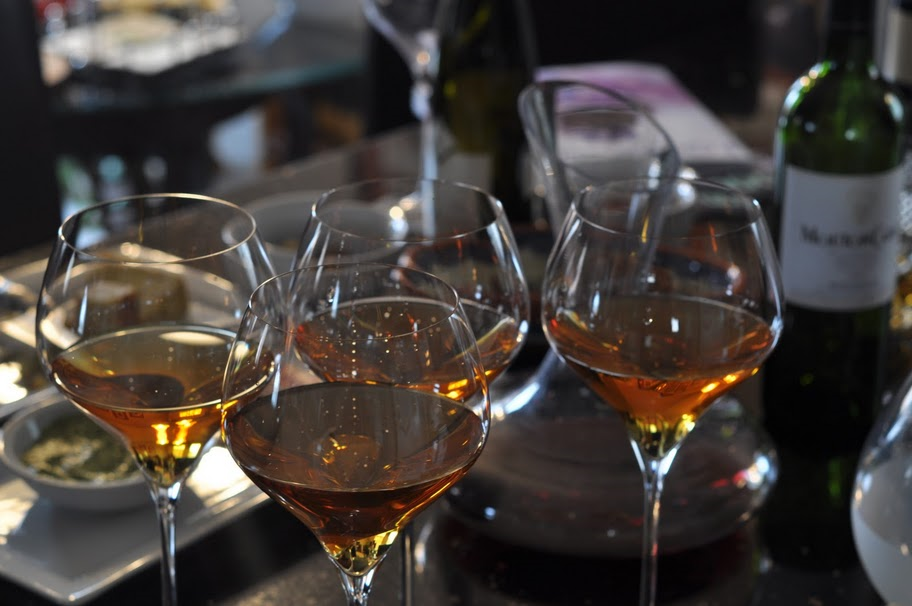
\includegraphics[width=0.5\textwidth]{wine}
%    \caption{16-year old white wine.}
%    \label{fig:wine}
%\end{figure}

The wine becomes deeper in colour going from a light yellow to golden.
\subsubsection{Another Sub-subsection}

% consistent table numbering in the report body
Some more text.  As a demonstration of tables, \Cref{tab:numbertable} demonstrates how certain types of entries should appear in a table.  Note that, in order to centre the numbers in the last column, three columns are given.

% tables have a number and title/caption above the table
\begin{table}[ht!] % h! means "here!" (instead of on top of the page)
    \caption{A table of numbers}
    \label{tab:numbertable}
    \centering
    \begin{tabular}{l r c r l S[table-format=5.4]}
        % 4.4 means 4 digits before and after the decimal point
        
        \hline
              & \multicolumn{1}{c}{\textbf{Integers}} & \multicolumn{1}{c}{\textbf{Boolean}} & \multicolumn{1}{c}{\textbf{Monetary}} & \multicolumn{1}{c}{\textbf{Text}} & \multicolumn{1}{c}{\textbf{Units (g/mL)}} \\
        \hline
        % ~ gives space
        Row 1 & 3~~~                                  & T                                    & 12.34                                 & First class                       & 0.1234                                    \\
        Row 2 & 9~~~                                  & F                                    & 5.67                                  & Some more text                    & 5.67                                      \\
        Row 3 & 23~~~                                 & F                                    & 890.12                                & Other text                        & 89.01                                     \\
        Row 4 & 157~~~                                & T                                    & 34.56                                 & Even more text                    & 23456.7                                   \\
        \hline
    \end{tabular}
\end{table}

\subsection{Another Subsection}

Some more text.

\subsection{A Third Subsection}

Some text and a reference to \Cref{app:anotherappx} which contains additional information related to this report.

\section{Background}

% consistent table numbering in the report body
The background of the report.  As another example, \Cref{tab:anothernumbertable} displays another set of numbers, but are actually the same as \Cref{tab:numbertable}.

% tables have a number and title/caption above the table
\begin{table}[ht!]
    \caption{Another table of numbers}
    \label{tab:anothernumbertable}
    \centering
    \begin{tabular}{l r c r l S[table-format=5.4]}
        % 4.4 means 4 digits before and after the decimal point
        
        \hline
              & \multicolumn{1}{c}{\textbf{Integers}} & \multicolumn{1}{c}{\textbf{Boolean}} & \multicolumn{1}{c}{\textbf{Monetary}} & \multicolumn{1}{c}{\textbf{Text}} & \multicolumn{1}{c}{\textbf{Units (g/mL)}} \\
        \hline
        Row 1 & 3~~~                                  & T                                    & 12.34                                 & First class                       & 0.1234                                    \\
        Row 2 & 9~~~                                  & F                                    & 5.67                                  & Some more text                    & 5.67                                      \\
        Row 3 & 23~~~                                 & F                                    & 890.12                                & Other text                        & 89.01                                     \\
        Row 4 & 157~~~                                & T                                    & 34.56                                 & Even more text                    & 23456.7                                   \\
        \hline
    \end{tabular}
\end{table}

\section{The Engineering Problem}

Some more text.

\section{Requirements, Criteria, and Metrics}

% add when necessary
\label{sec:rcm} % a label for "requirement, criteria, and metrics"

A list of the requirements, criteria and metrics that will be used in this report together with a discussion on any issues surrounding the selection of these.

This is an example of an inline equation: the formula $\sum_{n=1}^{\infty}\frac{1}{n^2}=\frac{\pi^{2}}{6}$ is often taught in first year.  The integral, however, is slightly less, as is shown by the display equation

\begin{center}
    $\int\limits_{1}^{\infty}\frac{1}{x^{2}}\, \mathrm{d}x=1$.
\end{center}

This is of course centred.

\section{Possible Solutions}

Equations can be numbered, for example, it may be necessary to refer to

\begin{equation}
    \label{eq:newtonssecondlaw}
    F=\frac{\mathrm{d}}{\mathrm{d}t}(m\mathbf{v}),
\end{equation}

that is, Newton\textquoteright s second law, elsewhere in the document.  Cut-and-paste this table if you require an equation elsewhere.

\subsection{Solution 1}

A description and discussion of solution 1 and a reference to \cref{eq:newtonssecondlaw}.

\subsection{Solution 2}

A description and discussion of solution 2.

\subsection{Solution 3}

A description and discussion of solution 3 and so on.

\section{Engineering Analysis}

The analysis of the solutions based on the requirements and criteria listed above based on the metrics listed in \Cref{sec:rcm} on \cpageref{sec:rcm}

\section*{Conclusions}

From the analysis in the report body, it was concluded that...

\section*{Recommendations}

Based on the analysis and conclusions in this report, it is recommended that...

%%%%%%%%%%%%%%%%%%%%%%%%%%%%%%%%%%%%%%%%%%%%%%%%%%%%%%%%%%%%%%%%%%%%%%%%%%%%%%%%
%% ************************************************************************** %%
%% *                                Glossary                                * %%
%% ************************************************************************** %%
%%%%%%%%%%%%%%%%%%%%%%%%%%%%%%%%%%%%%%%%%%%%%%%%%%%%%%%%%%%%%%%%%%%%%%%%%%%%%%%%

\printglossaries

%%%%%%%%%%%%%%%%%%%%%%%%%%%%%%%%%%%%%%%%%%%%%%%%%%%%%%%%%%%%%%%%%%%%%%%%%%%%%%%%
%% ************************************************************************** %%
%% *                               References                               * %%
%% ************************************************************************** %%
%%%%%%%%%%%%%%%%%%%%%%%%%%%%%%%%%%%%%%%%%%%%%%%%%%%%%%%%%%%%%%%%%%%%%%%%%%%%%%%%

\printbibliography[heading=none]

%%%%%%%%%%%%%%%%%%%%%%%%%%%%%%%%%%%%%%%%%%%%%%%%%%%%%%%%%%%%%%%%%%%%%%%%%%%%%%%%
%% ************************************************************************** %%
%% *                               Appendices                               * %%
%% ************************************************************************** %%
%%%%%%%%%%%%%%%%%%%%%%%%%%%%%%%%%%%%%%%%%%%%%%%%%%%%%%%%%%%%%%%%%%%%%%%%%%%%%%%%

% appendices use section and subsection numbering
\appendix

\section{Title of First Appendix}
\label{app:firstappx}
Use the No Spacing style.

\section{Another Appendix}
\label{app:anotherappx}
Again, use the no spacing style for appendices.

\end{document}

